\chapter{Related work}

\section{Referential framework}

\subsection{Spectrogram}
A spectrogram is a three-dimensional representation of the spectral content of the speech signal. It represents the power of the different spectral components of each instance of speech.

Spectrograms are images that represent sequences of spectra. Spectrogram is computed with Fourier Transform (FT) to transform a time domain signal into frequency domain signal. The whole signal is divided into individual windows(signal portions) and the FT is calculated for each window and join them back into a single image that shows the dominant frequencies in
each window \cite{sribhashyam2021pattern, wyse2017audio} as is shown in the figure \ref{fig:spectrogram}.

\begin{figure}
    \centering
    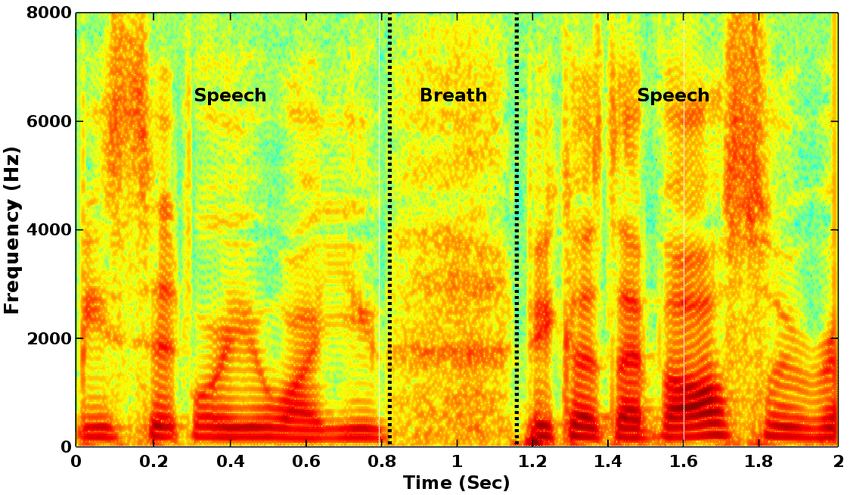
\includegraphics[height=8cm]{figures/spectogram.png}
    \caption{Spectrogram of a speech signal with breath sound (marked as Breath), whose bounds are denoted by vertical dotted lines.}
    \label{fig:spectrogram}
\end{figure}


\subsection{Formants}
The formants of speech are resonant regions within the spectrogram. The vocal tract is changing shape so that the resonance is changing. the vocal tract length is inversely proportional to the height of the format in the frequency range of a speaker

Literature also showed that there are differences between male and female voices. The average female formant and fundamental frequencies are higher than that of the male speaking voice \cite{wu1991gender}. Formants are a frequency range where there is an absolute or relative maximum in the sound spectrum. The frequency at the maximum is the formant frequency\cite{pierce2019acoustics}. First formant, F1 corresponds to the vertical position of the tongue and is associated with frequencies between 200 and 900 Hz. Second formant, F2 corresponds to the horizontal position of the tongue and ranges from 600 - 2600 Hz \cite{watson1998acoustic}.

\subsection{Vowel space}
The vowel space is a two-dimensional area bounded by the first and second formant frequency coordinates of vowels \cite{sandoval2013automatic}. The \ac{VSA}, defined as the area of the quadrilateral formed by the four corner vowels when projected on the first two formant frequencies (F1 and F2), is often used to characterize speech motor control \cite{berisha2014characterizing} as is shown in the figure \ref{fig:vowel}. one method to use is the analysis of the vowel space during speech model training, thereby providing the foundational knowledge for developing a method to visualise and evaluate speech synthesis model training\cite{abeysinghe2022visualising}.

\begin{figure}
    \centering
    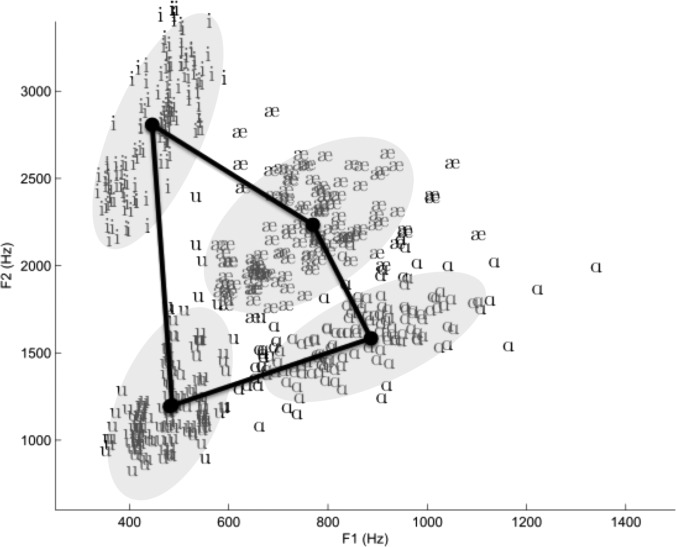
\includegraphics[height=6cm]{figures/vowel_space.png}
    \caption{The distribution of the first two formant frequencies for the four corner vowels that define the area of the vowel space.}
    \label{fig:vowel}
\end{figure}

\subsection{Error metrics and EER}

the classifier computes a score $r$ for the 
input trial and compares $r$ with a threshold $\tau$. The trial is classified as being
bonafide if $r \geq \tau$, otherwise
spoofed, two types of classification error can occur:

\begin{itemize}
    \item False rejection: falsely classifying a bona fide trial as being spoofed.
    \item False acceptance: falsely classifying a spoofed trial as being bona fide.
\end{itemize}

Without loss of generality, let us use \(p_{bona}(r;\theta)\) and \(P_{spoof}(r;\theta)\) to denote the score distributions of the bona fide and spoofed trials in a dataset, respectively.
The \(\theta\) denotes the trained parameter set of the PAD model. figure \ref{fig:error} illustrates examples of the score distributions. The classification threshold \(\tau\) marks the
region to claim bonafide and spoof. The shaded area of \(P_{bona}(r;\theta)\) on the left
side of \(\tau\) denotes false rejection. In contrast, the area of \(P_{spoof}(r;\theta)\) on the right side of \(\tau\) denotes false acceptance. Accordingly, the false rejection rate (FRR) and false acceptance rate (FAR) can be computed as 

\begin{equation}
    FRR(\tau) = \int_{-\infty}^{\tau} P_{bona}(r;\theta) \,dr
\end{equation}

\begin{equation}
    FAR(\tau) = \int_{\tau}^{\infty} P_{spoofed}(r;\theta) \,dr
\end{equation}

While being informative, the DET curve is not handy when a single metric is desired. One metric to summarize the discriminative power of the PAD model is the EER. In theory, EER refers to the joint between the DET curve and the anti-diagonal line (see the middle circle on the DET curve in \ref{fig:error}). In practice the EER can be computed by:

\begin{equation}
    EER = \frac{FRR(\tau^{\prime}) + FAR(\tau^{\prime})}{2}
\end{equation}

\begin{equation}
    \tau^{\prime} = \underset{\tau}{\mathrm{arg min}} \ |FRR(\tau)-FAR(\tau)|
\end{equation}

\begin{figure}
    \centering
    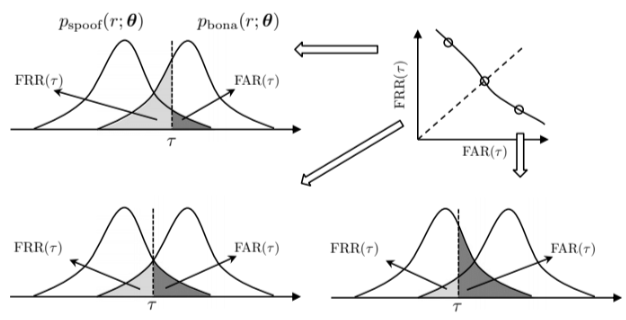
\includegraphics{figures/eer.png}
    \caption{ Illustration of FRR($\tau$), FAR($\tau$), and DET curve.}
    \label{fig:error}
\end{figure}



\section{State of the art}

\subsection{Speaker recognition}
Speech is an acoustic output produced by precisely coordinated movement of different human body parts. Therefore, there have been suggestions that acoustic features of speech can convey information about the physical characteristics of the speaker\cite{gupta2022estimation}.

\subsection{Logical Access Presentation Attack}

Presentation attack mounted at the transmission point can use \ac{TTS} or \ac{VC} systems to produce the speech waveform of a target speaker (i.e., victim). While the algorithms vary in detail, both \acs{TTS} and \acs{VC} can be written as a mapping function that converts one data sequence into another\cite{wang2022practical}. They can use specific models to convert the input into an acoustic feature for instance a sequence to convert the input text into a Mel-spectrogram \cite{shen2018natural}.

\subsection{Font End}

\subsubsection{DSP-based Deterministic Approaches}

Many front ends are based on \ac{DSP} algorithms that extract a sequence of acoustic features. Many speech processing tasks have used \ac{MFCC} \cite{davis1980comparison}. \ac{LFCC} \cite{davis1980comparison} and \ac{IMFCC} are closed related to the MFCC, but they use a different frequency scale and emphasize different frequency bands of the input waveform. Another popular front end is the \ac{CQCC} that uses \ac{CQT} rather than \ac{STFT}. Both \acs{CQCC} and \acs{LFCC} have been used in the ASVspoof challenges and are open-sourced. Rather than using cepstrum coefficients, many front ends only extract the spectrogram. Different from the cepstrum coefficients, \ac{LFB} compresses the spectrogram without cepstral analysis\cite{wang2022practical}.

\subsubsection{NN-based Supervised Training Approach}

\ac{DNN} can be used as a front end Different from a DSP-based one,  DNN-based front end has to be learned from the data. Such a trainable front end is preferred for three reasons. First, the DNN could be configured to extract acoustic features from a longer waveform segment. Second, the data-driven DNN with non-linear transformations is more powerful than linear operations in DSP-based front ends. Third, a DNN-based front end can easily be integrated with a DSP-based front end\cite{wang2022practical}. 

\subsubsection{DNN-based Self-supervised Training Approach}

It is also possible to apply self-supervised training to the DNN-based front end. One advantage is that a large amount of data can be used even if they do not have target labels. This is a popular topic in speech processing community, and many models have been proposed: wav2vec \cite{schneider2019wav2vec}, wav2vec2 \cite{baevski2020wav2vec}, VQ-wav2vec \cite{baevski2019vq},
contrastive predictive coding \cite{chung2021similarity}, auto-regressive predictive coding \cite{chung2021similarity}, and
HuBERT \cite{hsu2021hubert, wang2022practical}. 


\subsection{Back End}

\subsubsection{DNNs with Discriminative Training}

Many advanced PAD models use DNN-based back ends. A major sub-category is a \acs{DNN} with a discriminative training strategy. Given the target label \(y\) of input waveform  \(o_{1:T}\), the \acs{DNN} is directly trained to maximize the probability \(P(y|o_{1:T};\theta_{3})\). We use \(\theta_3\) to denote the parameter set of the DNN-based back end so that it can be differentiated from \((\theta_{1},\theta_{2})\) of the DNN-based front end. The topology of the DNN is a designer’s choice\cite{wang2022practical}.

\subsection{End-to-end Models}

End-to-end models as a combination of a neural back end and a dummy front end. From another viewpoint, we can also split an end-to-end model into front and back ends. The term ‘end-to-end’ is based on the fact that the front and back ends are jointly trained\cite{wang2022practical}.

\endinput

